\subsection{Datasets}
Accurate point clouds are crucial to ensure that the predictions made by the model are built upon a reliable foundation. To generate synthetic “perfect” point clouds, parametric geometries were created in SolidWorks, introducing various shapes composed of simple geometries (see Figure \ref{fig:part_shapes_grid}). The parametric definitions of these geometries allow for the creation of numerous variations for each shape, resulting in a vast amount of data. Specifically, each part is represented in four different variations. These geometries are then converted into point clouds using \texttt{MeshLab}. A Poisson disc sampling technique is employed to ensure that the point clouds are uniformly distributed. To further enhance the robustness of the model, imperfections are deliberately introduced into the point clouds. By creating holes within the generated point clouds, the dataset will contain a mixture of points that are perfect and points that are in a low surface density area. 

After pointclouds are generated, features are extracted for each pointcloud using the method described in Section \ref{sec:features}. The labels are calculated by extracting the surface area of the parts from Solidworks and dividing it by the number of points in the pointcloud. This label is attached to all points in the pointcloud and only changed for points that are next to a generated hole. For points next to a hole, the surface density is halved to better match the ground truth quality of the point neighborhood.

The method was used to generate two datasets:
\begin{itemize}
    \item \textbf{Dataset 1 (Coarse mesh sampling)}: Mesh sizes of 0.5\,mm, 1\,mm, and 2\,mm were used for sampling the geometries, resulting in a dataset of 1,562,211 points.
    
    \item \textbf{Dataset 2 (Fine mesh sampling)}: Mesh sizes from 0.5\,mm to 2\,mm were generated at 0.1\,mm intervals, producing a finely sampled dataset of 4,950,604 points. This dataset allows the model to experience a smooth transition in mesh resolution, enhancing its ability to handle diverse point densities.
\end{itemize}


\begin{figure}[htbp]
  \centering
  \begin{minipage}{0.5\textwidth} % Half page width
    \centering
    \setlength{\tabcolsep}{1pt}
    \renewcommand{\arraystretch}{0.9}

    \begin{tabular}{ccc}
      \begin{minipage}{0.3\linewidth}
        \centering
        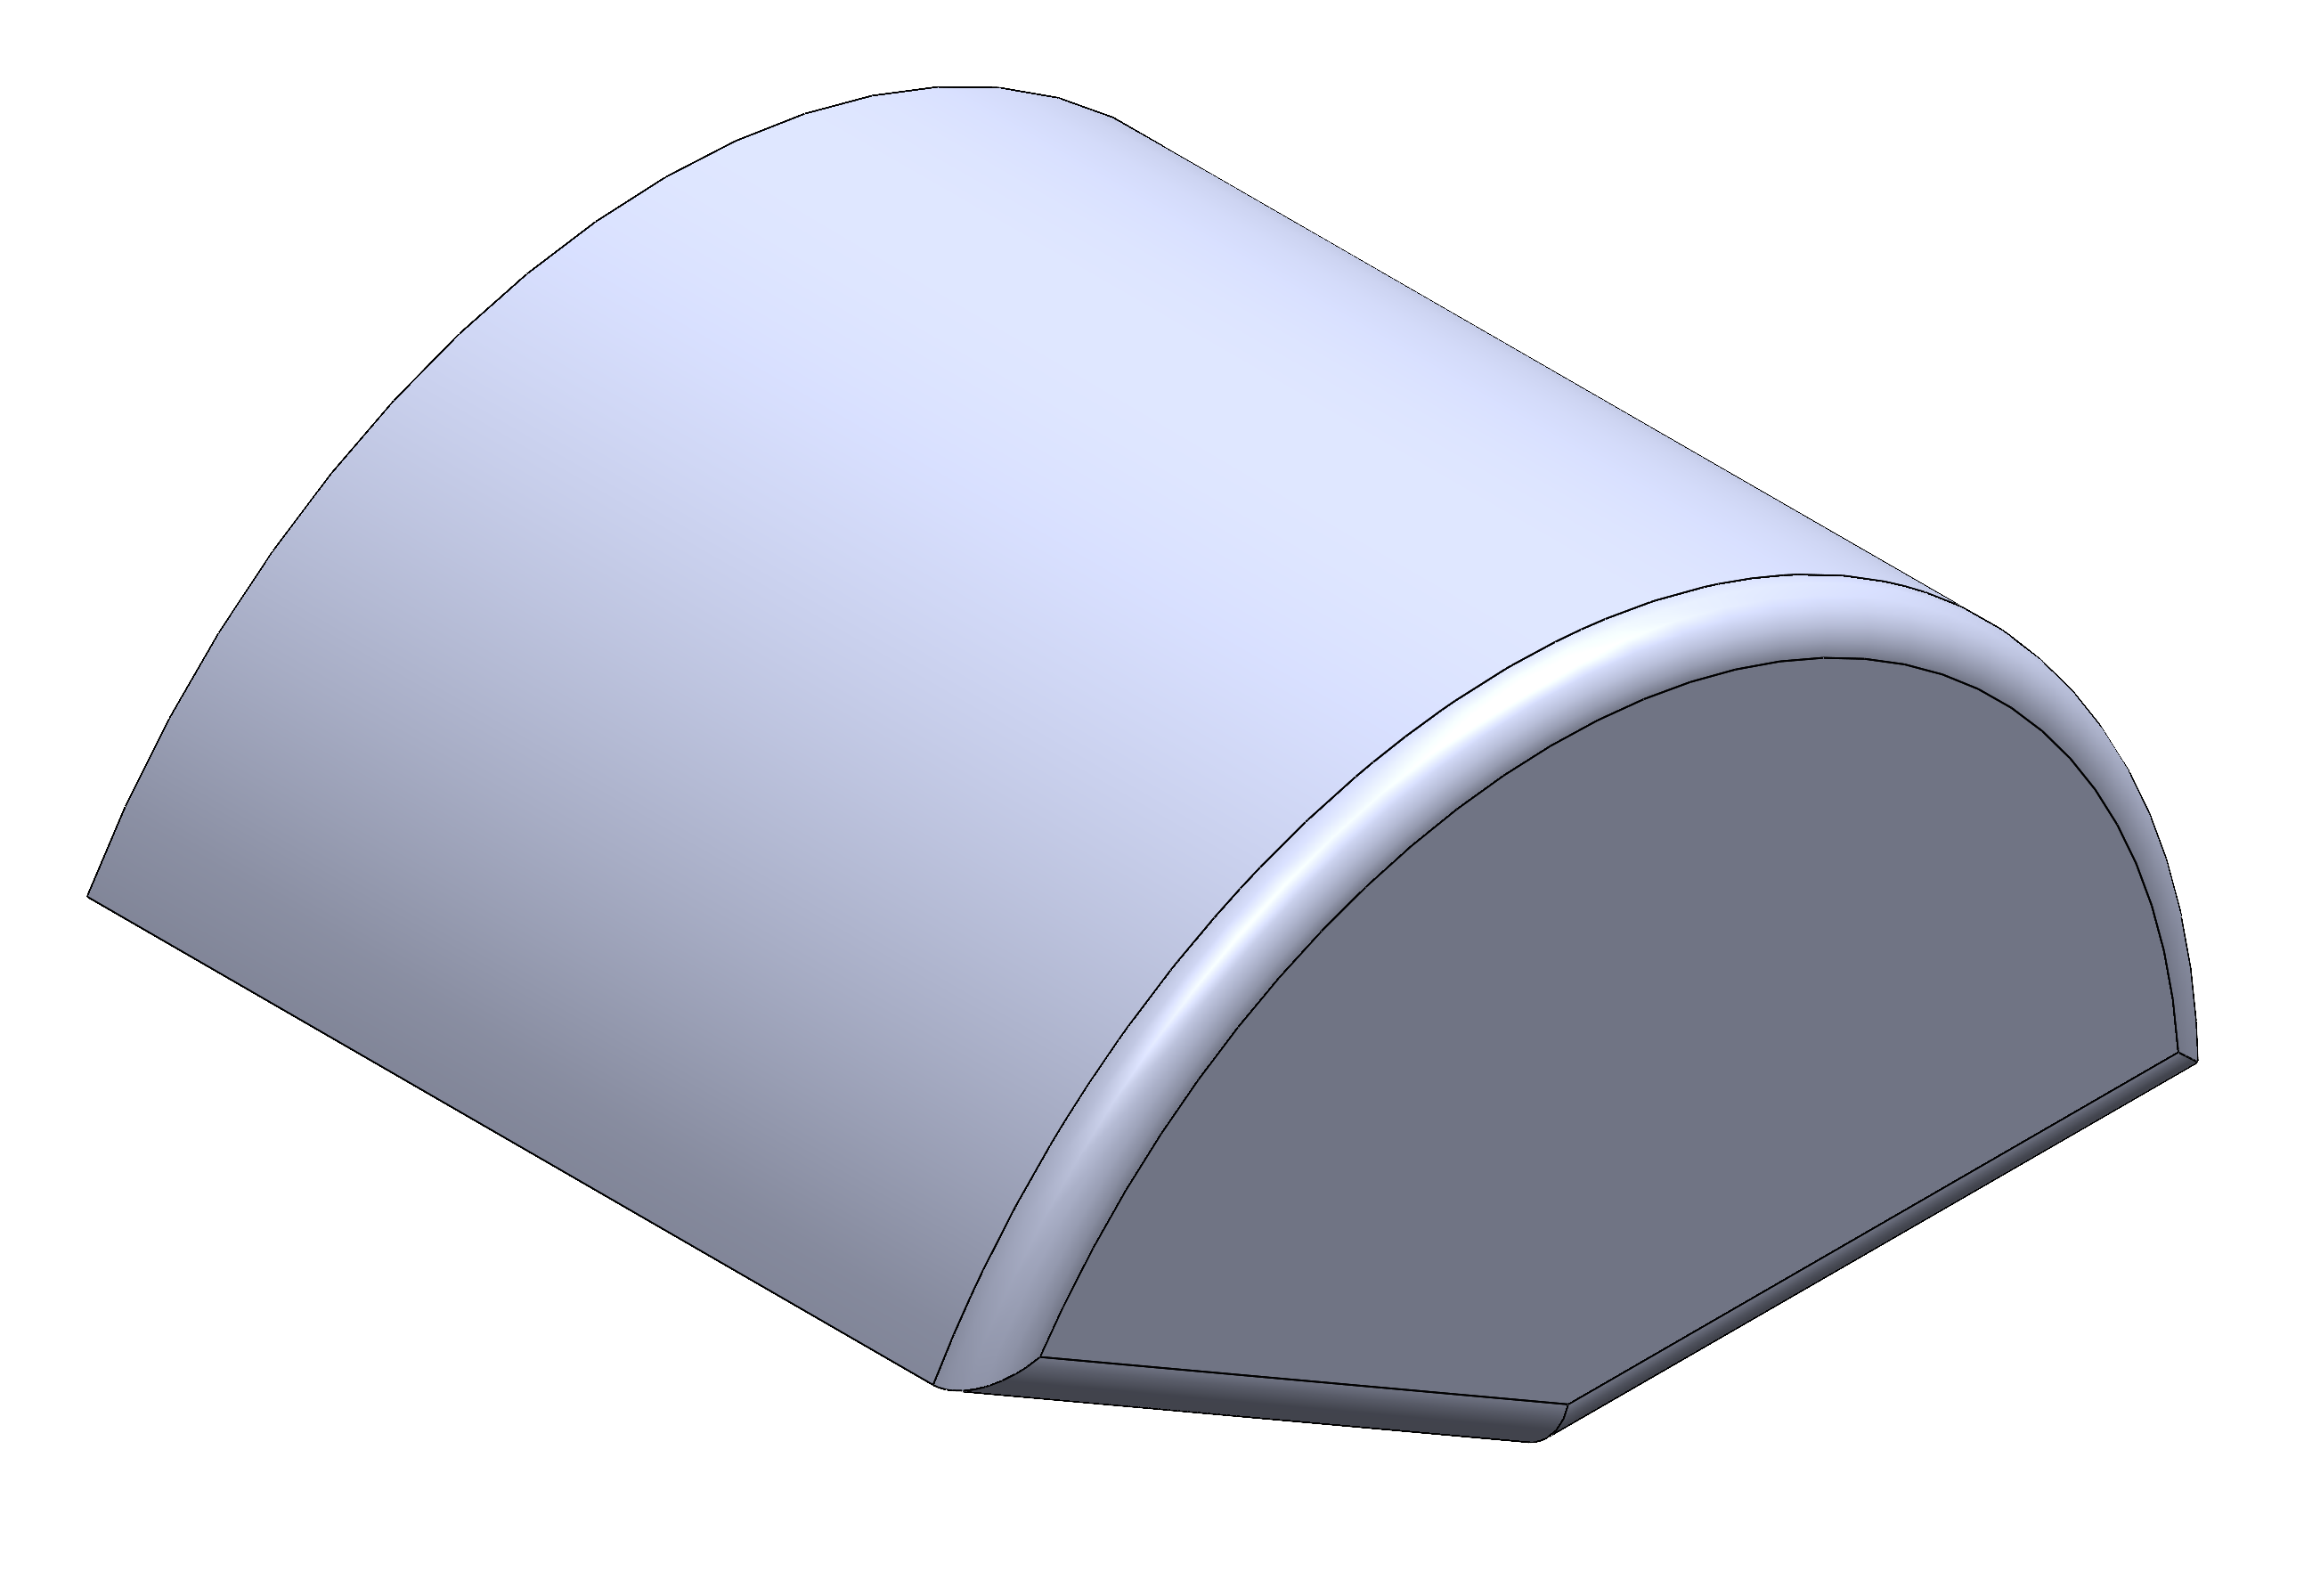
\includegraphics[width=\linewidth]{figures/parts/angle_curve.PNG}
        \scriptsize Angle Curve
      \end{minipage} &
      \begin{minipage}{0.3\linewidth}
        \centering
        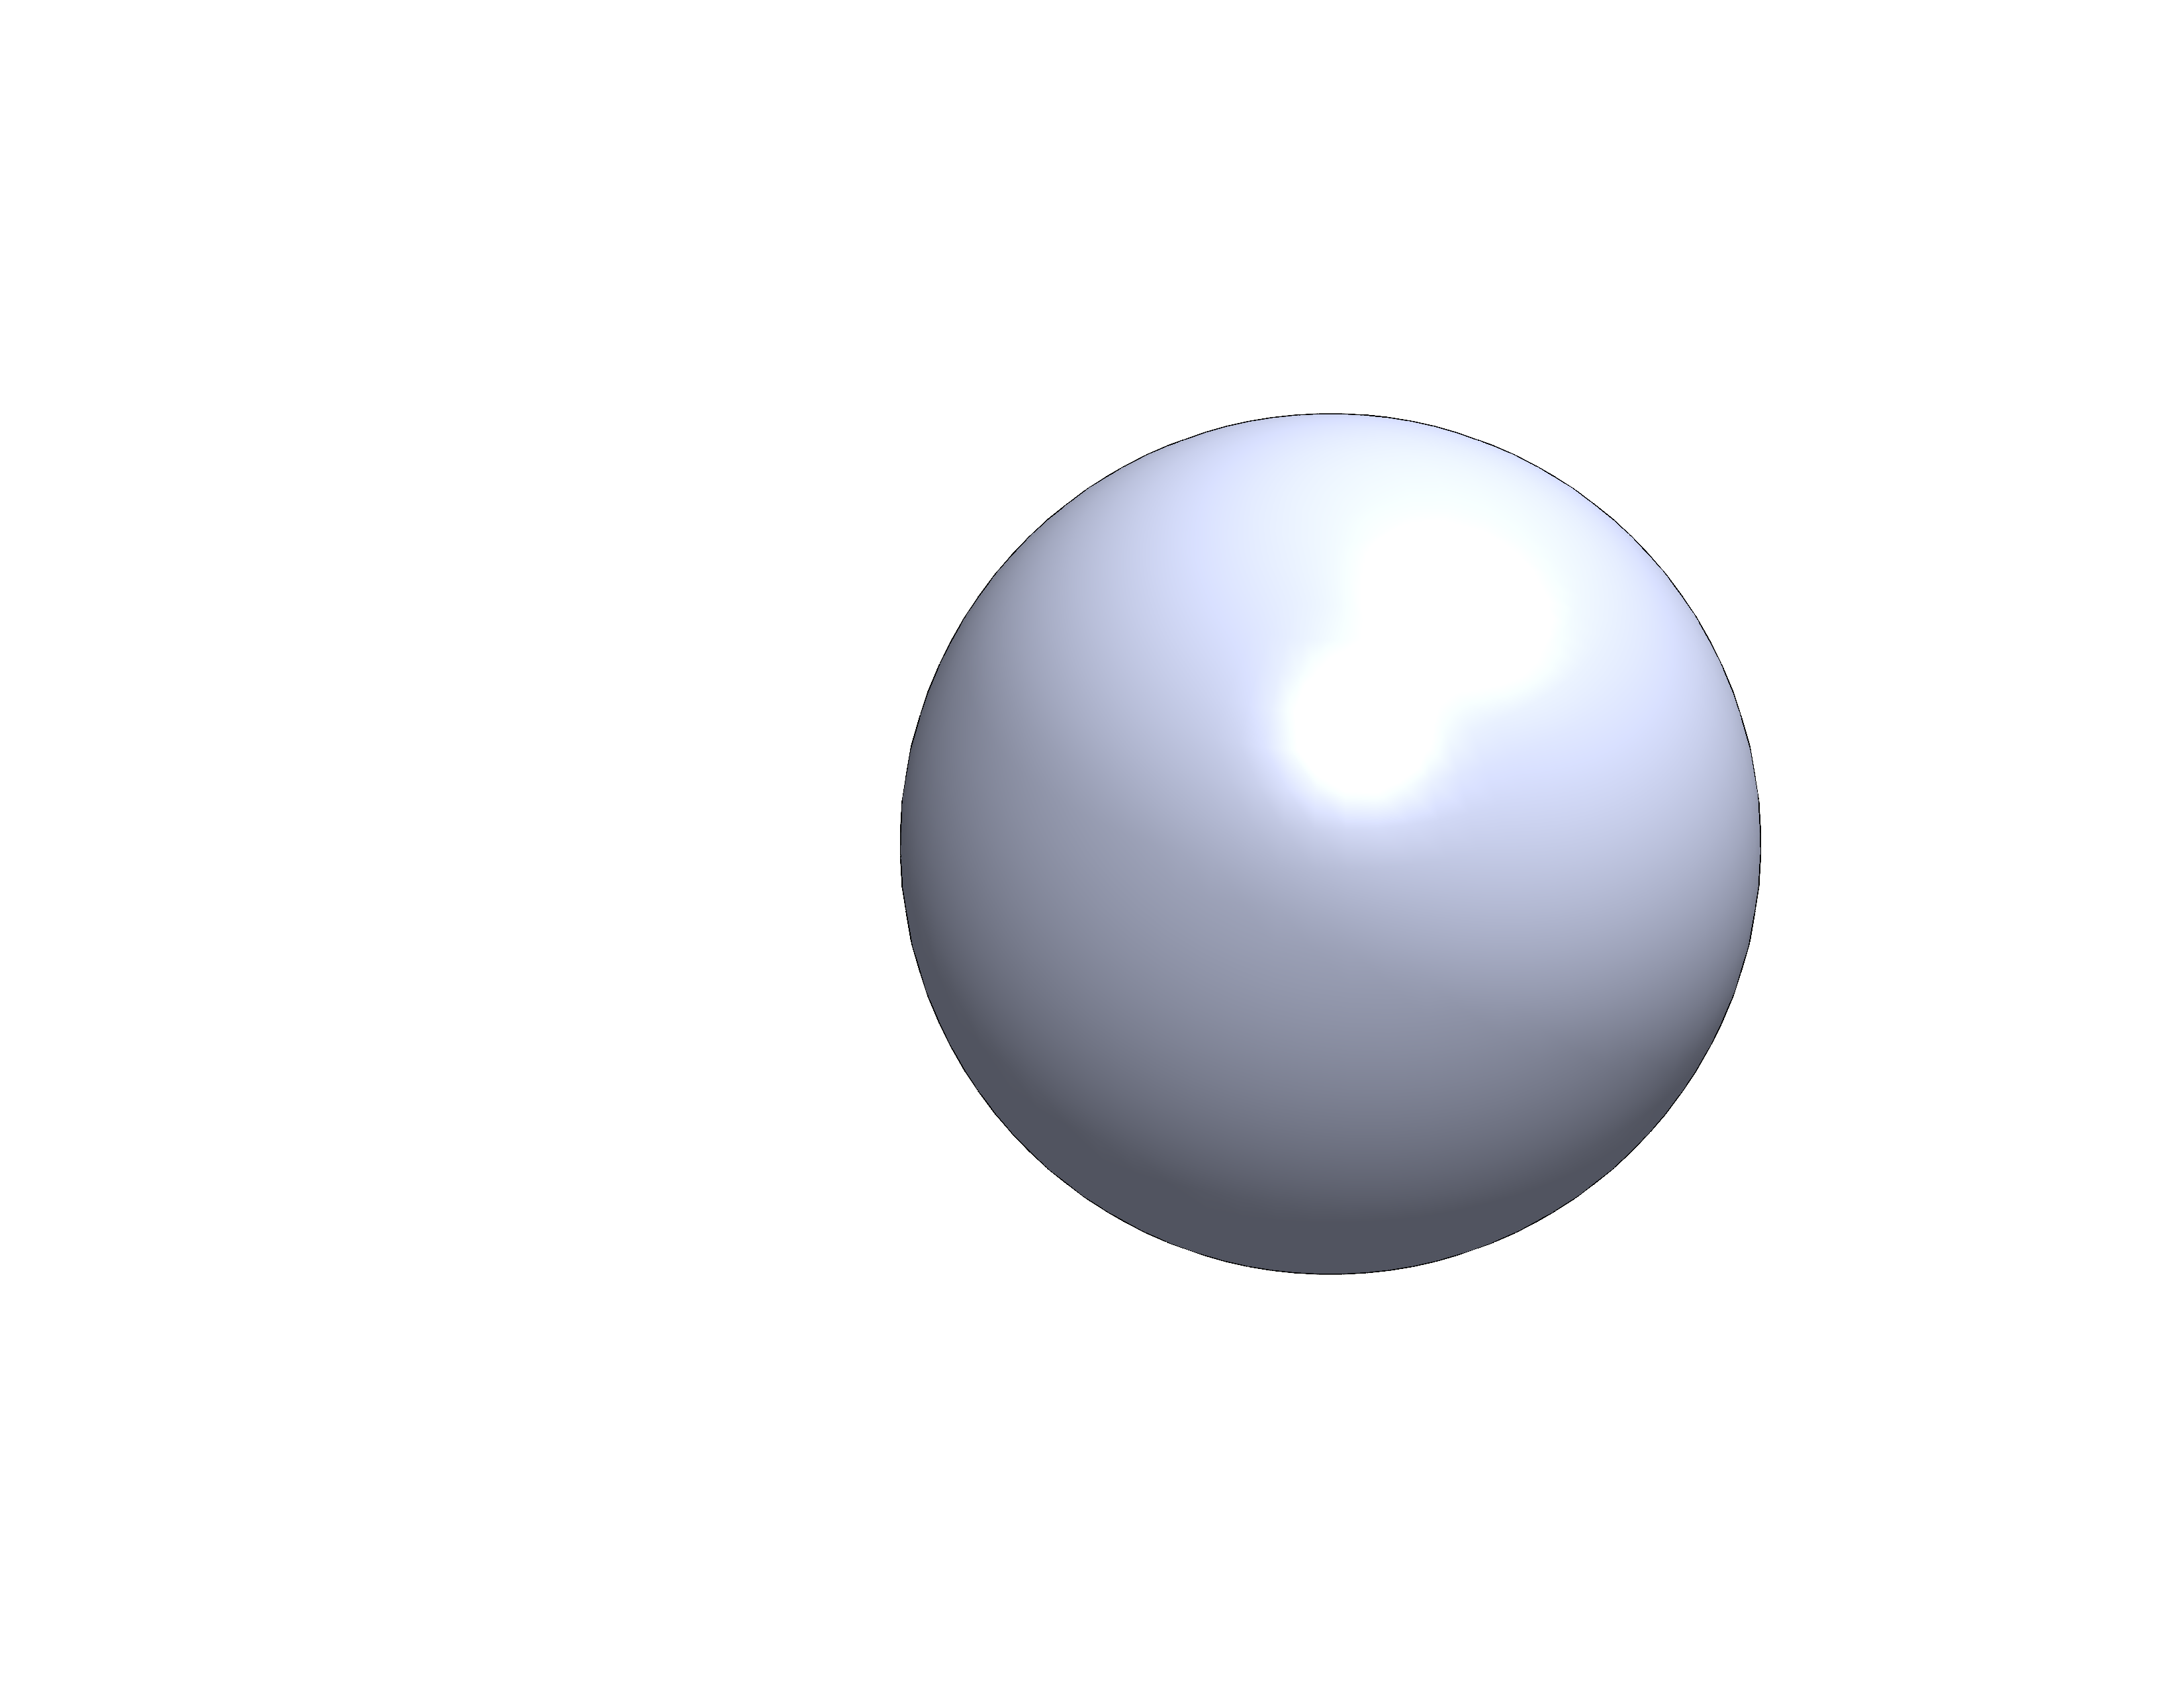
\includegraphics[width=\linewidth]{figures/parts/Ball.PNG}
        \scriptsize     Ball
      \end{minipage} &
      \begin{minipage}{0.3\linewidth}
        \centering
        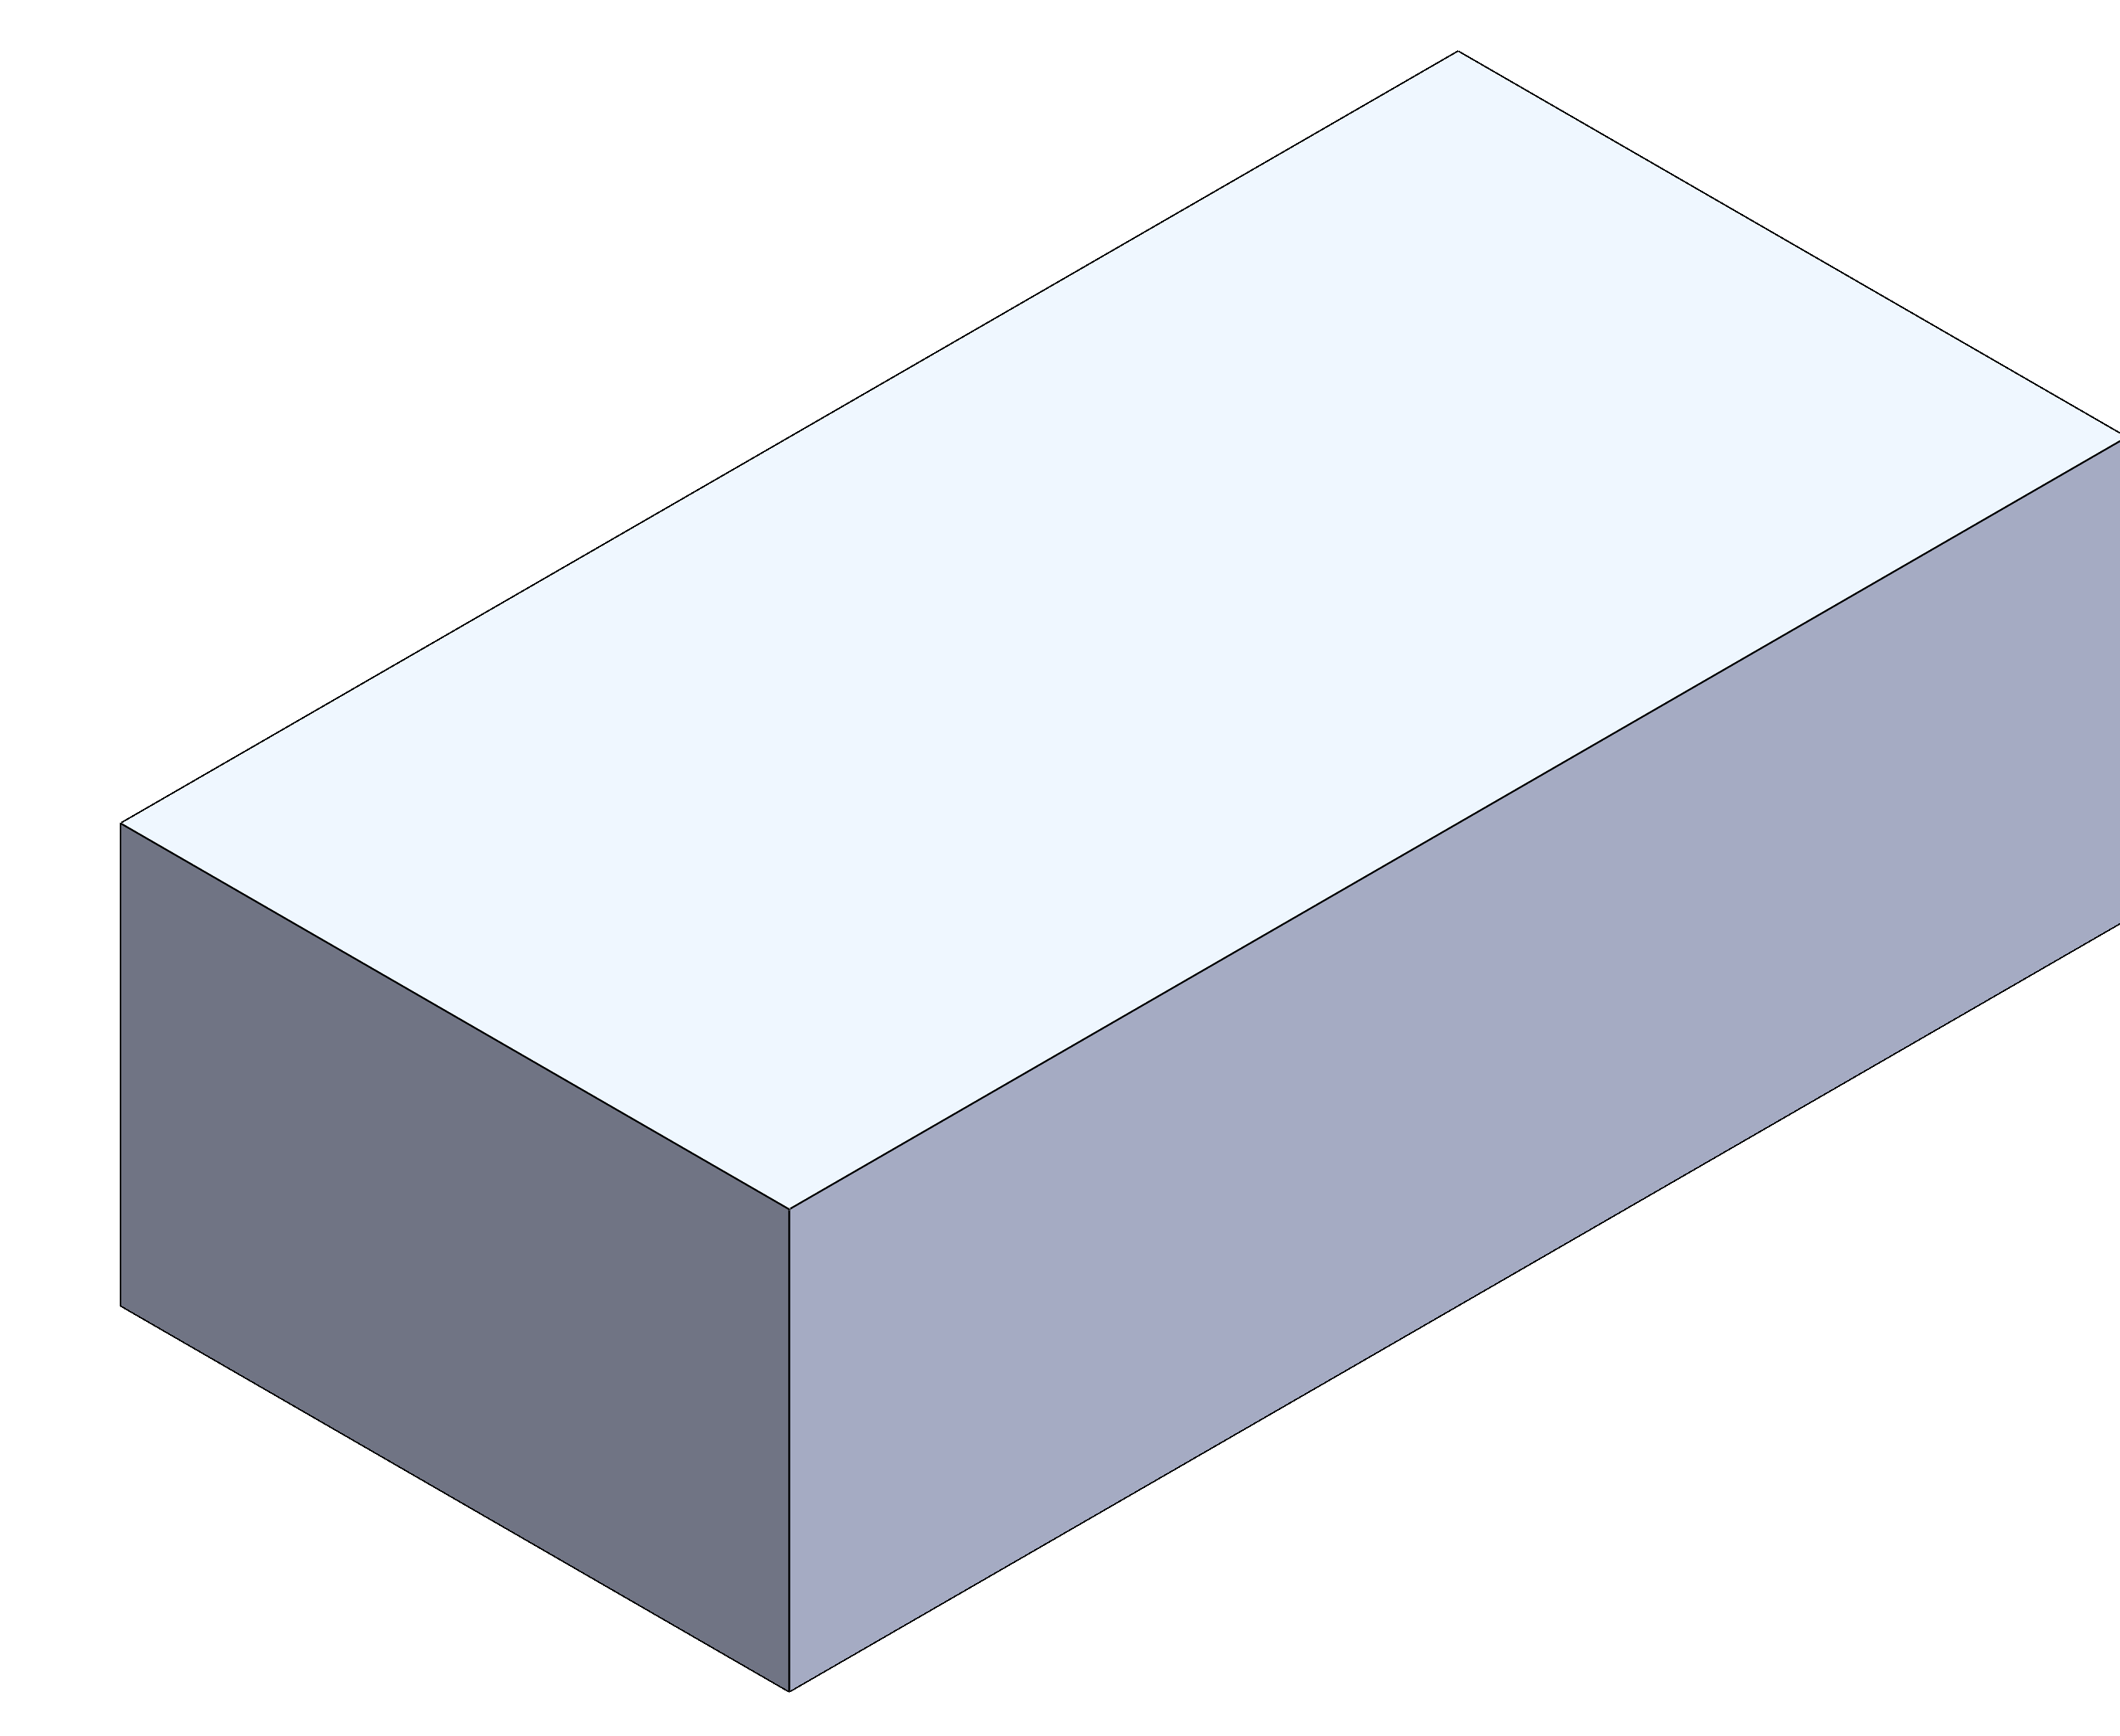
\includegraphics[width=\linewidth]{figures/parts/Box.PNG}
        \scriptsize Box
      \end{minipage} \\

      \begin{minipage}{0.3\linewidth}
        \centering
        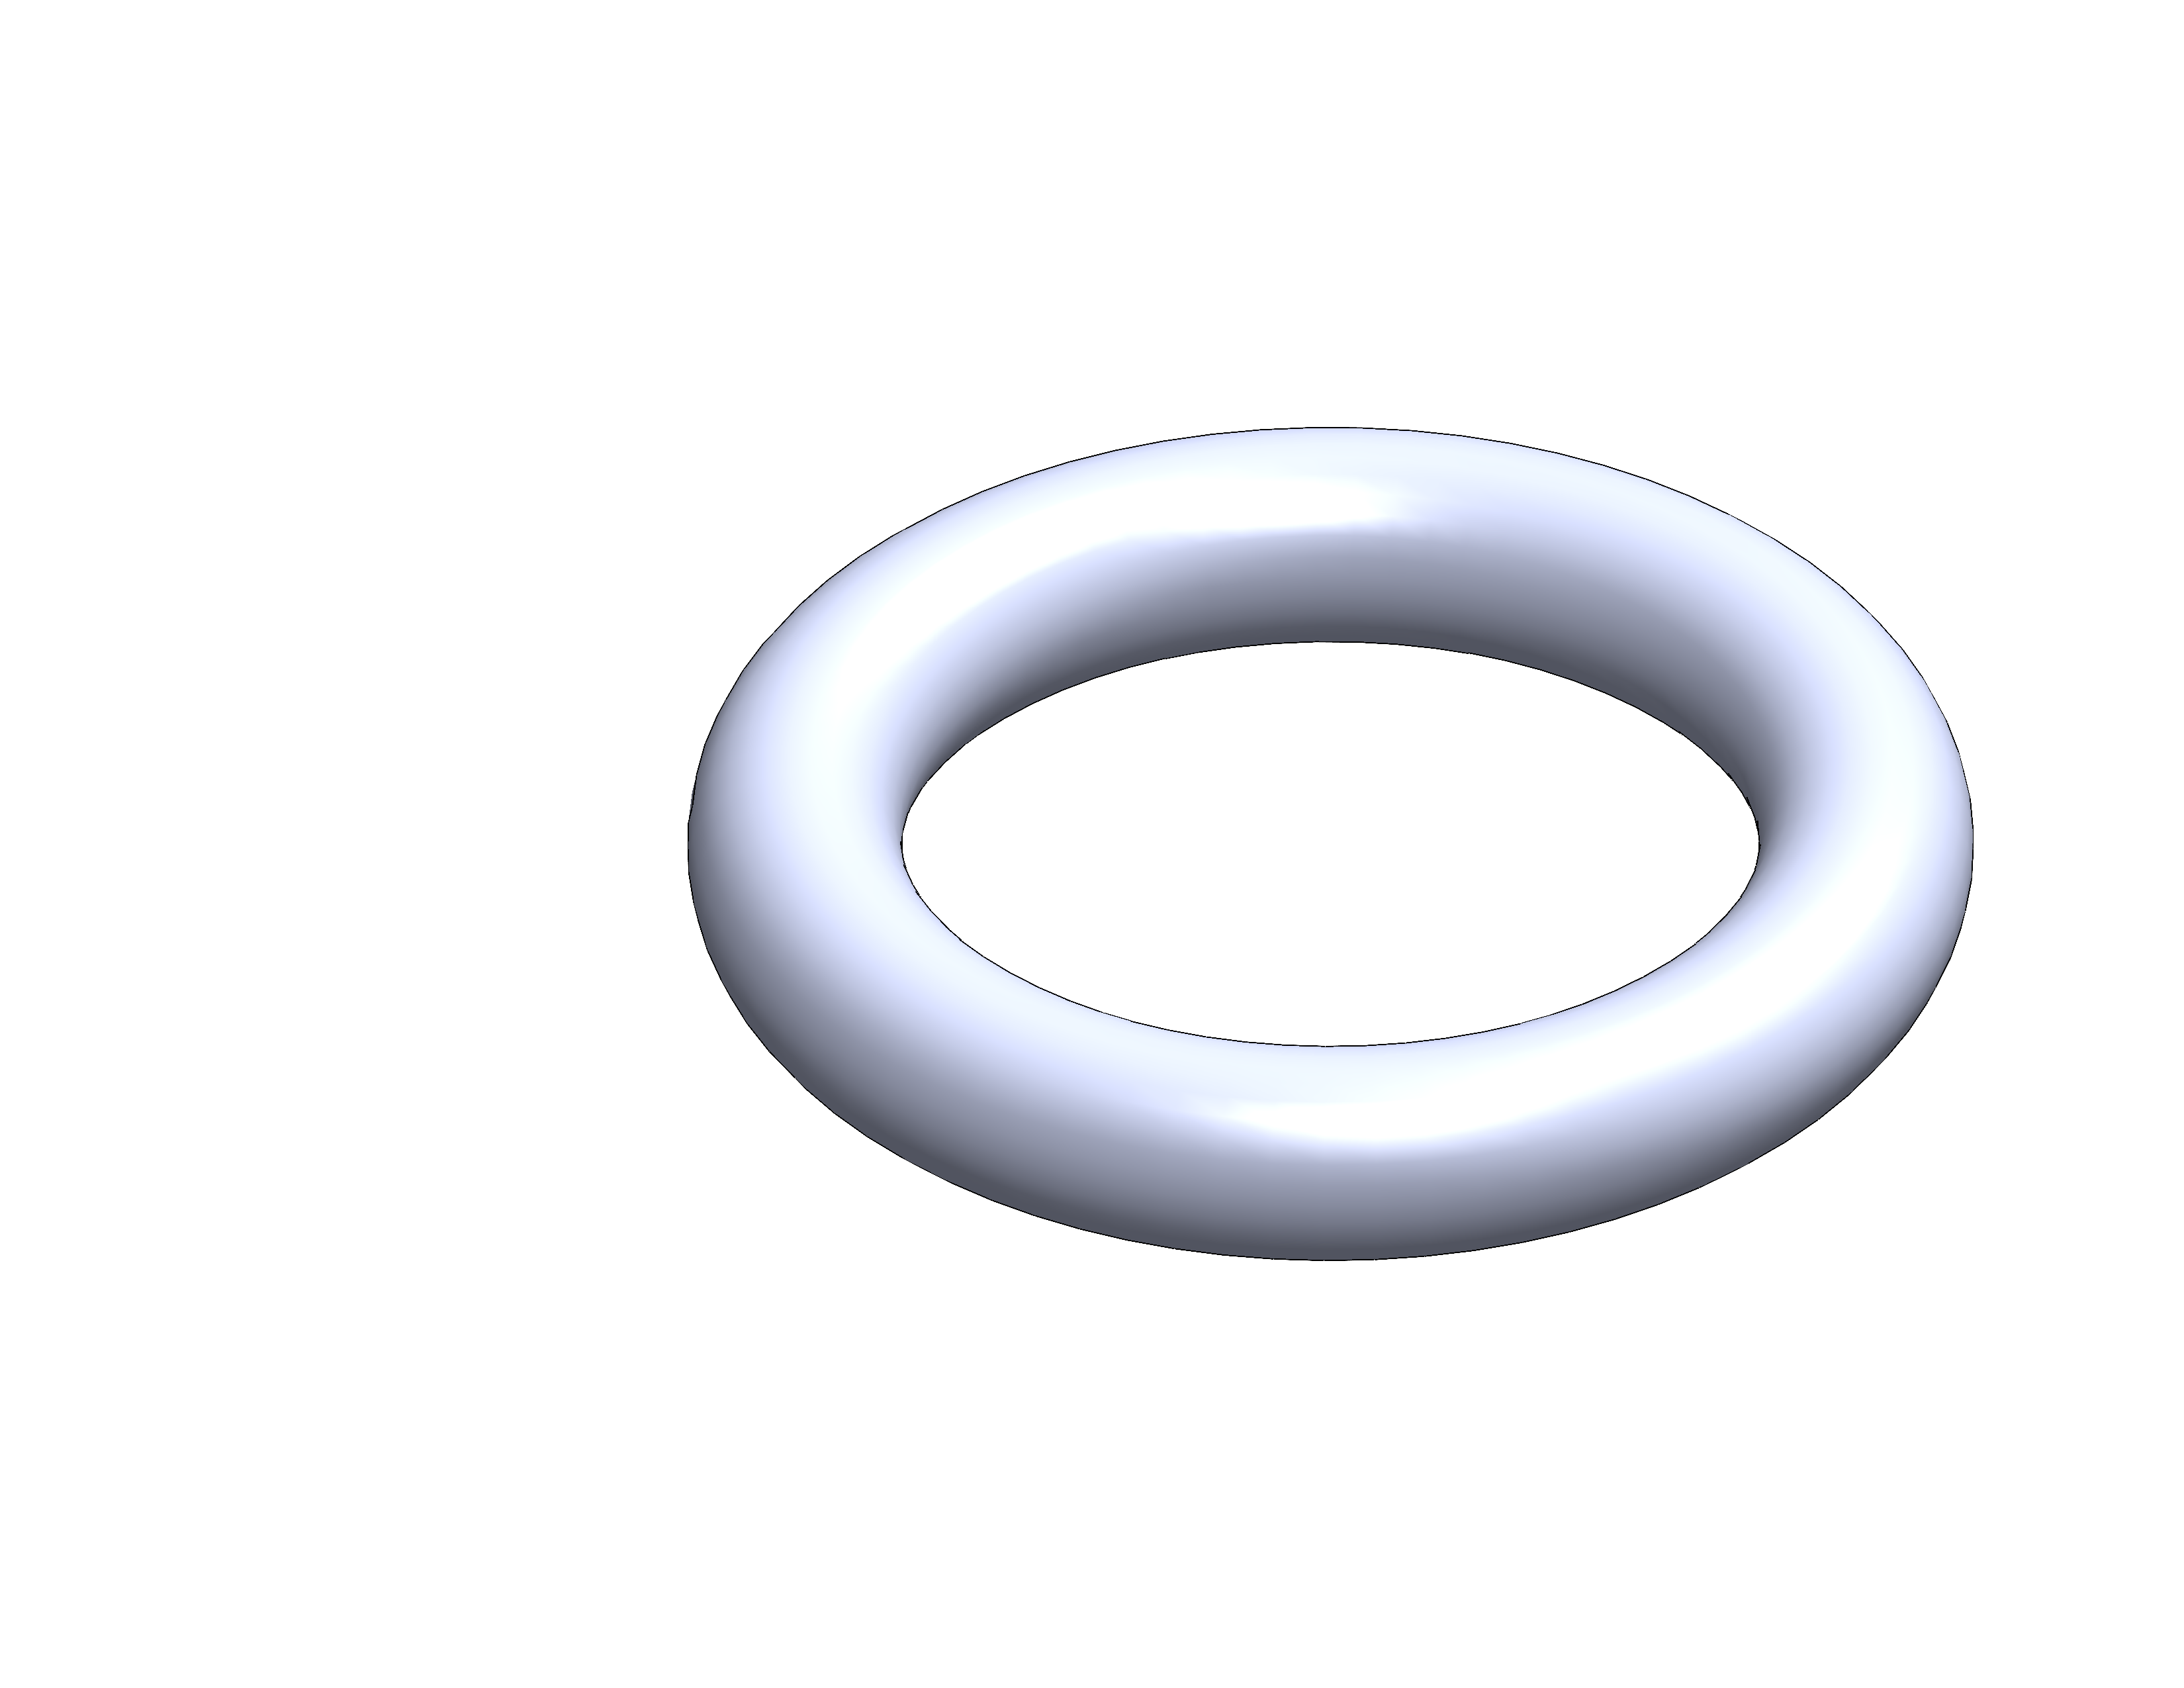
\includegraphics[width=\linewidth]{figures/parts/donut.PNG}
        \scriptsize Donut
      \end{minipage} &
      \begin{minipage}{0.3\linewidth}
        \centering
        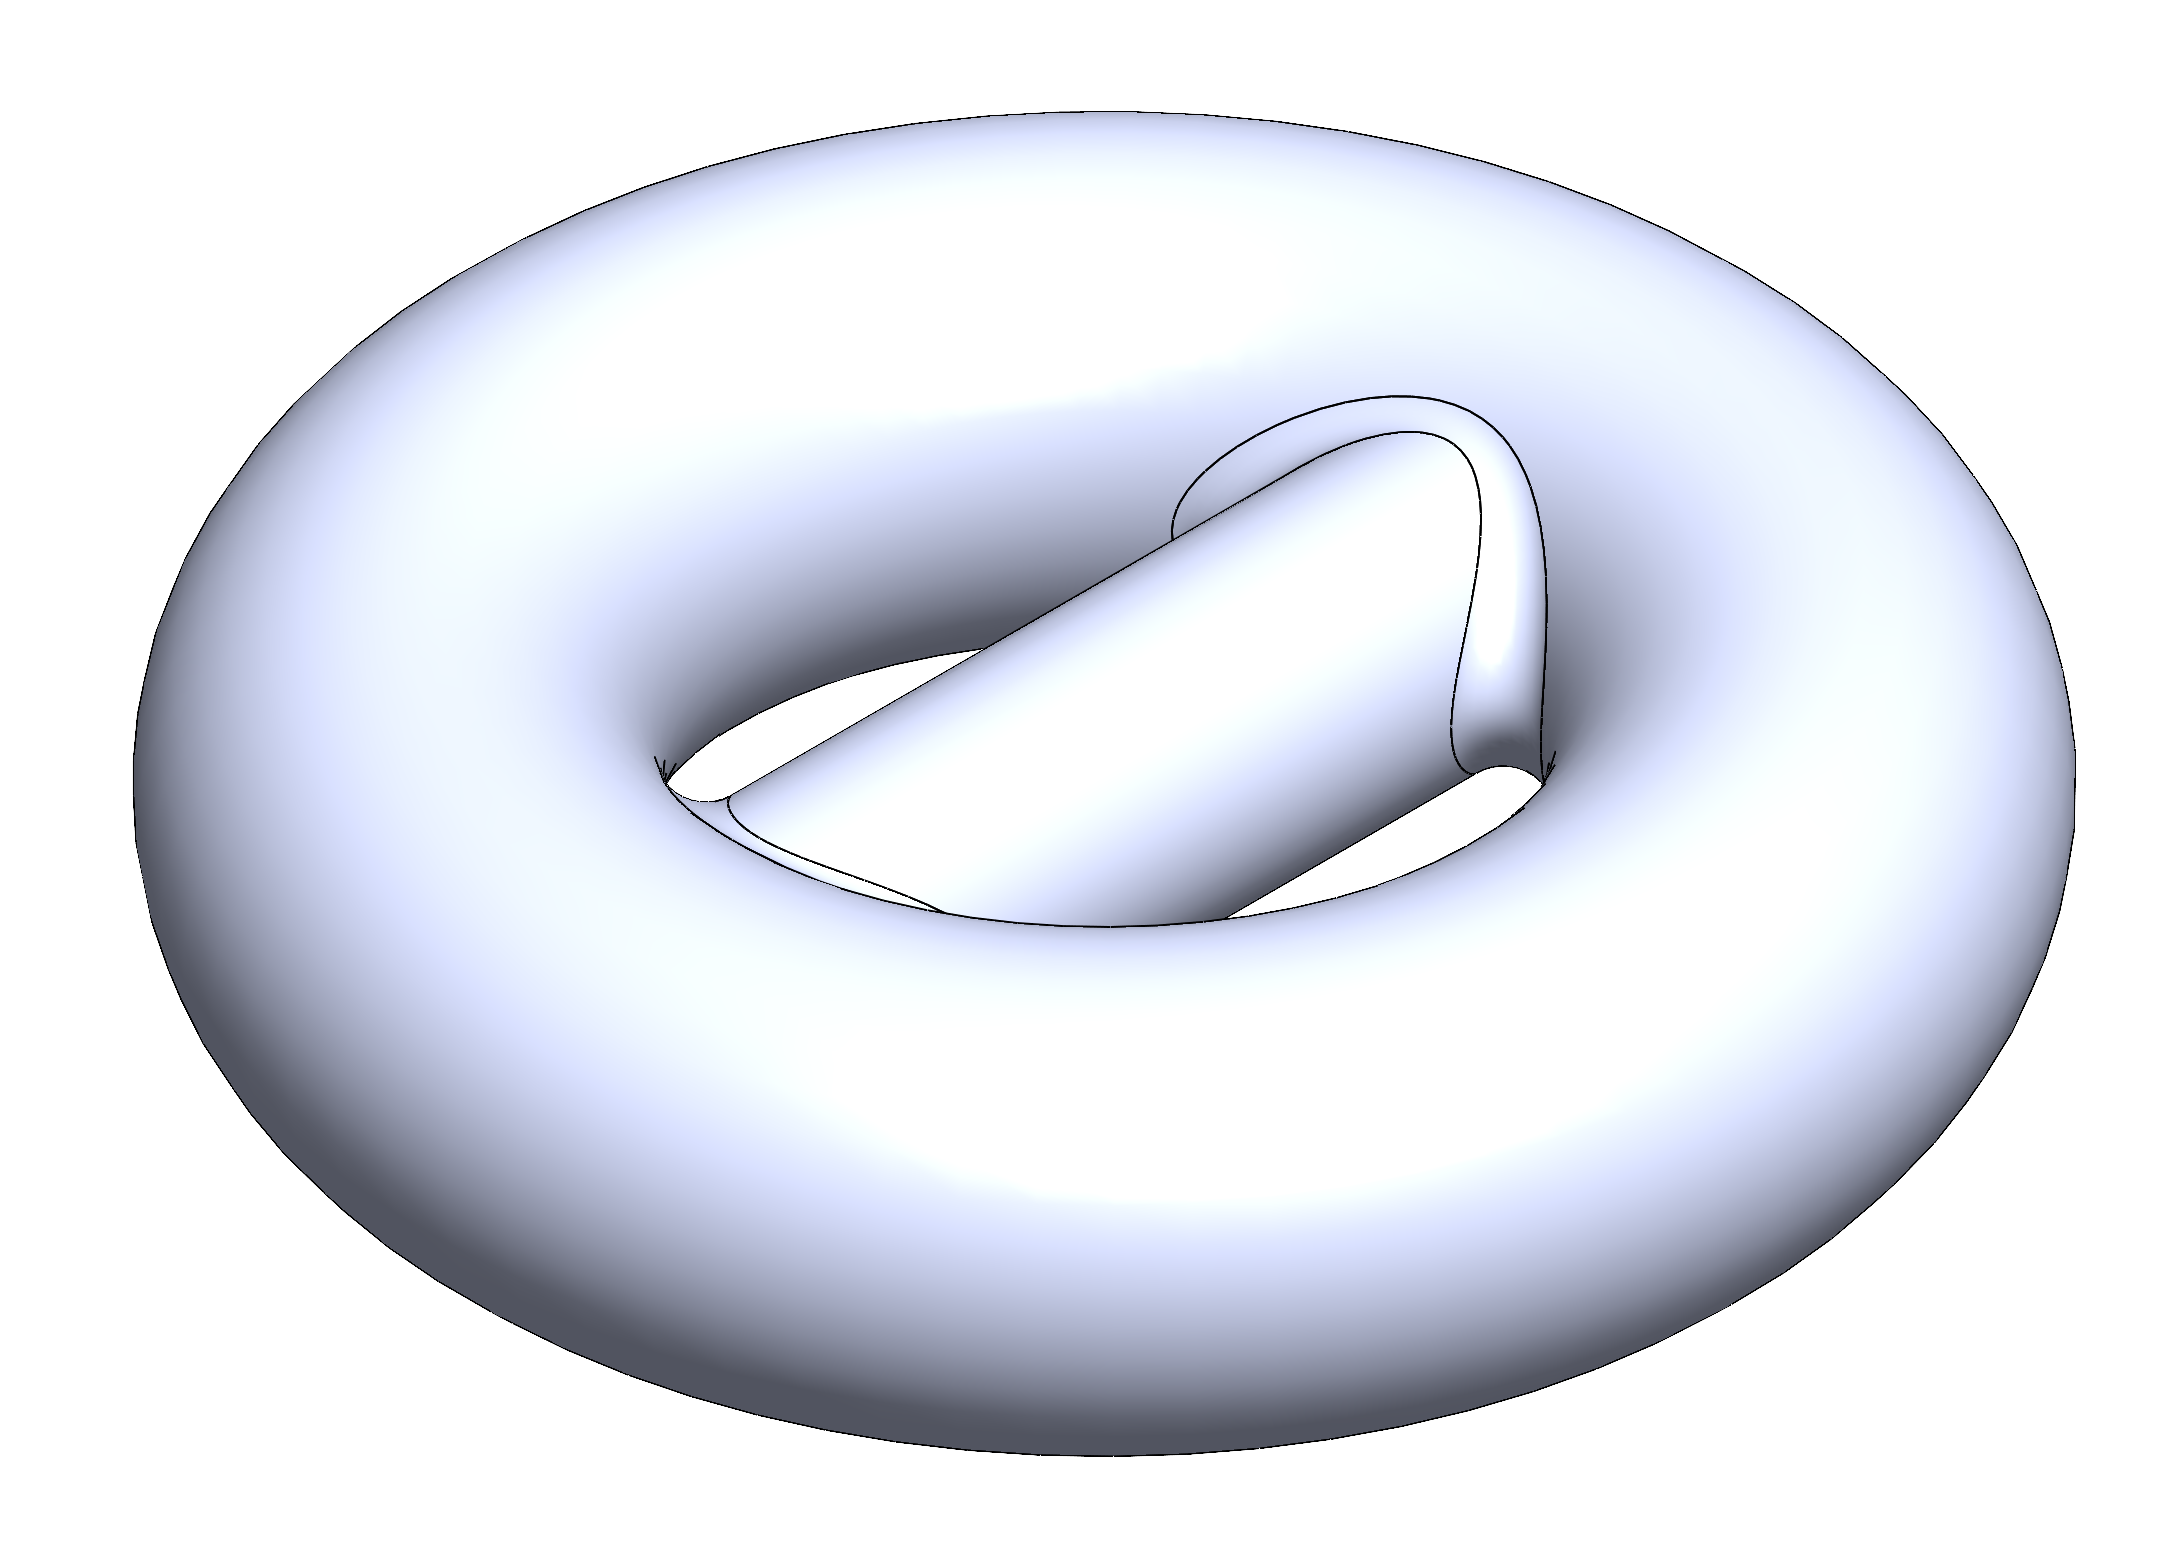
\includegraphics[width=\linewidth]{figures/parts/Donut_w_center.PNG}
        \scriptsize Donut w/ Center
      \end{minipage} &
      \begin{minipage}{0.3\linewidth}
        \centering
        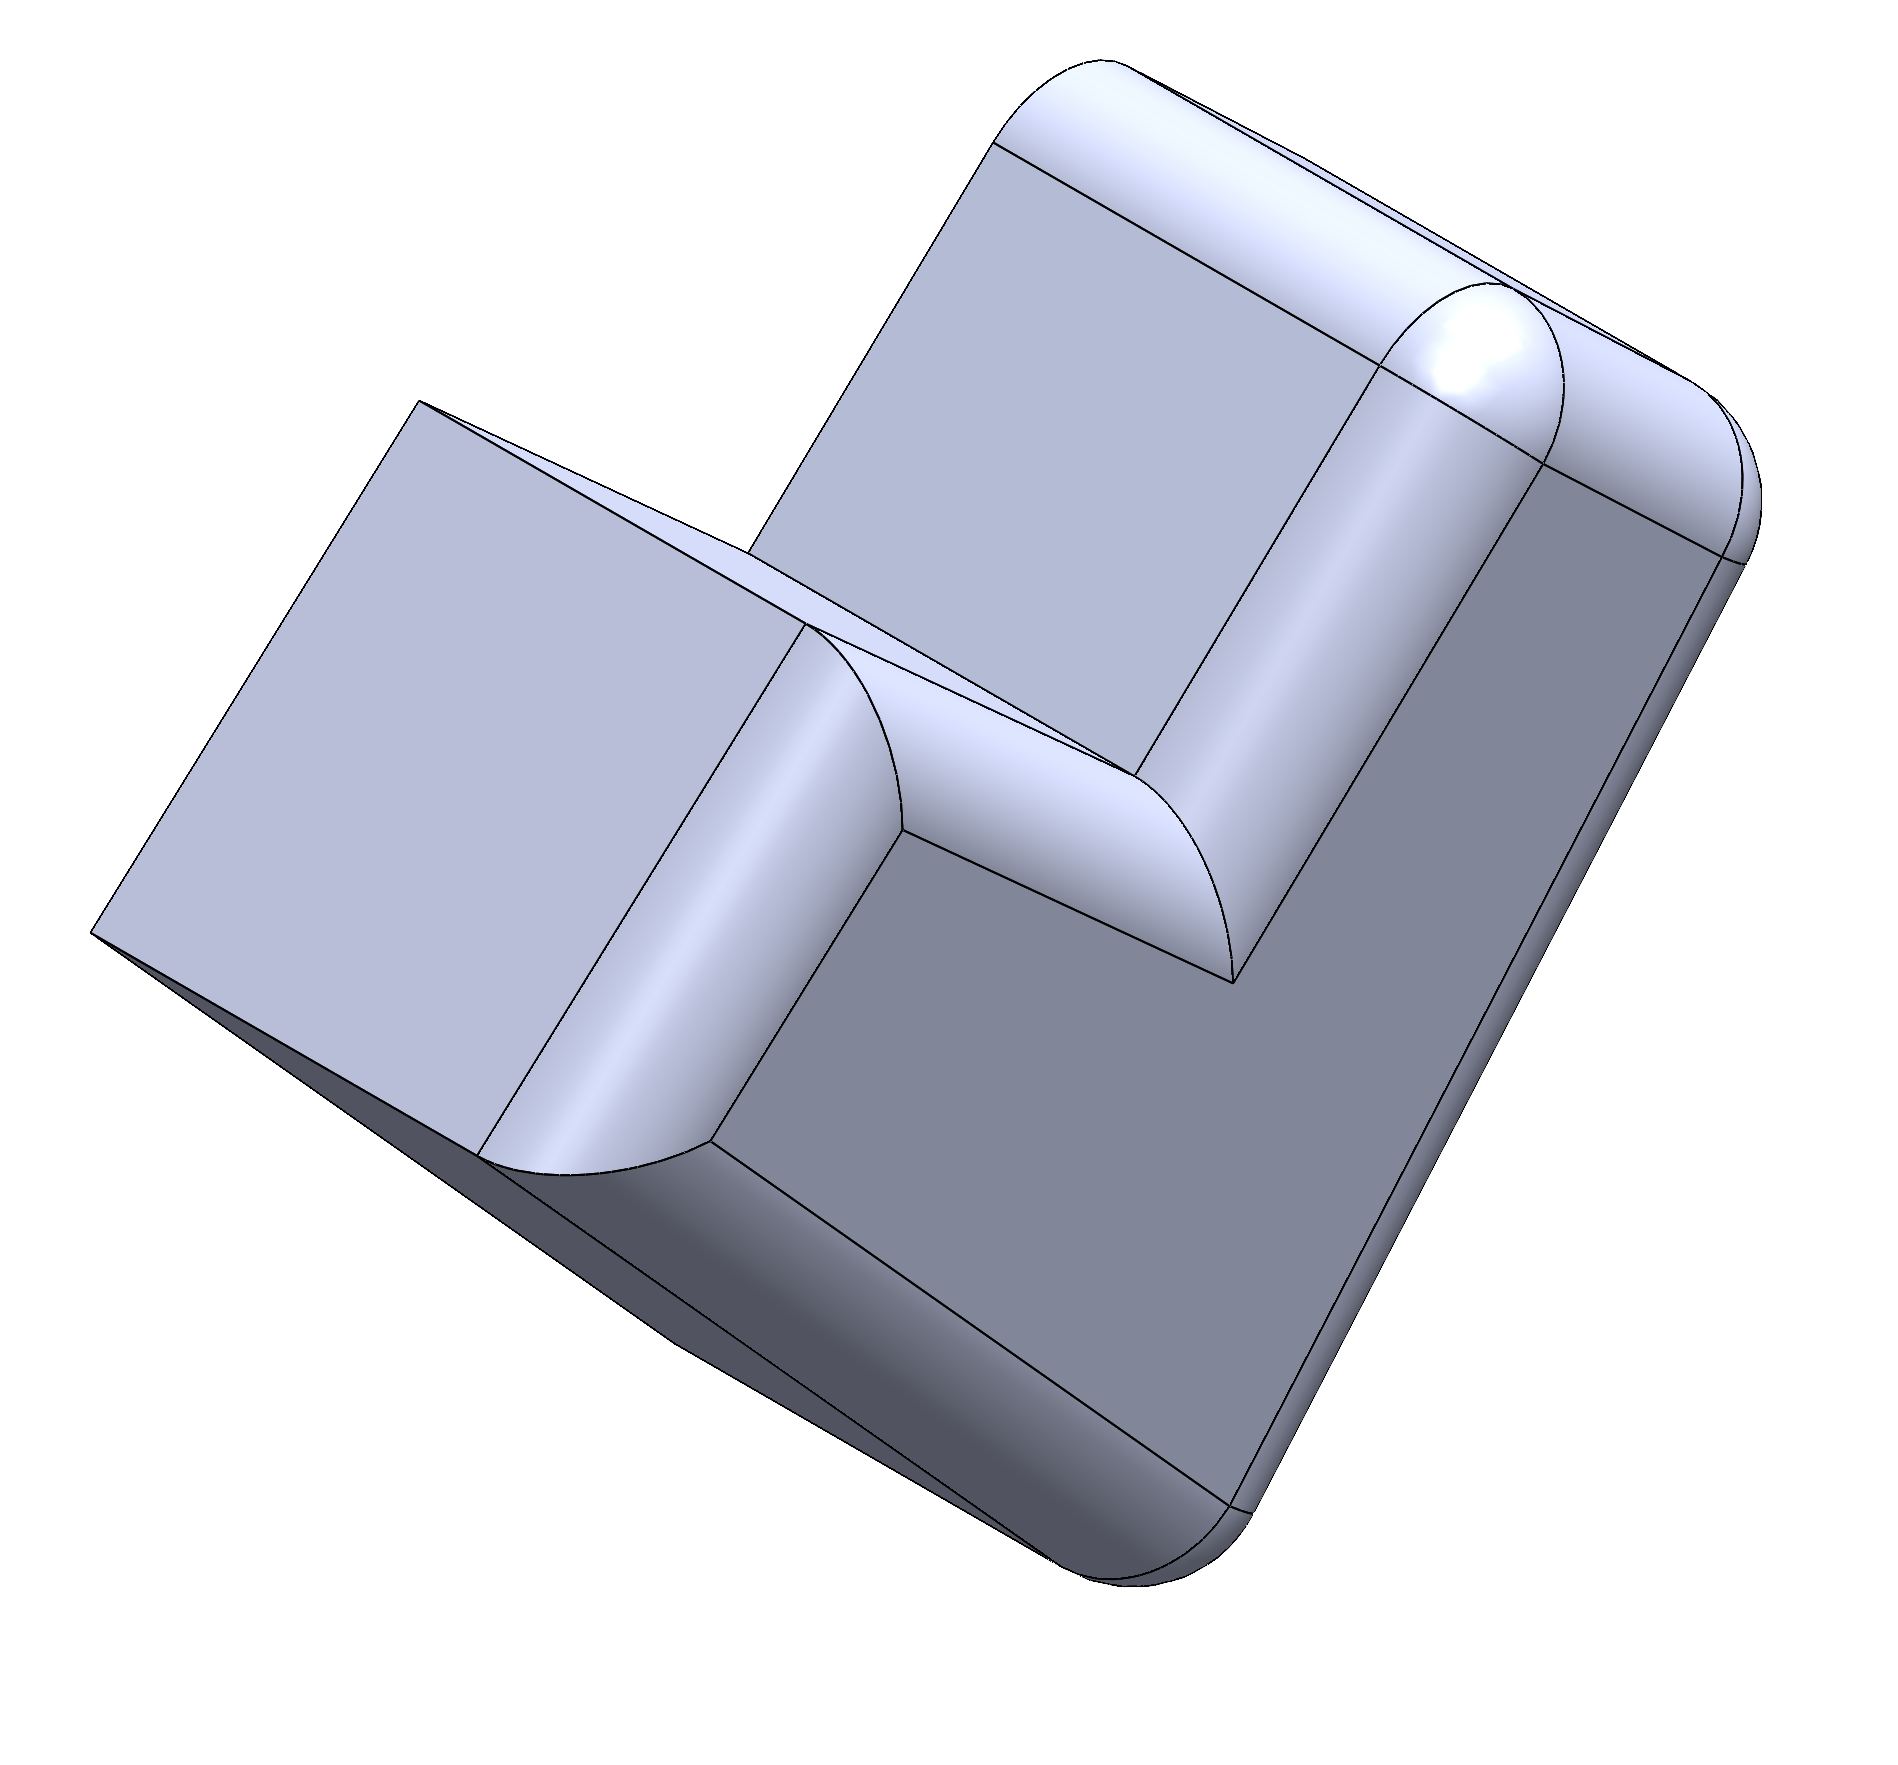
\includegraphics[width=\linewidth]{figures/parts/heart.PNG}
        \scriptsize Heart
      \end{minipage} \\

      \begin{minipage}{0.3\linewidth}
        \centering
        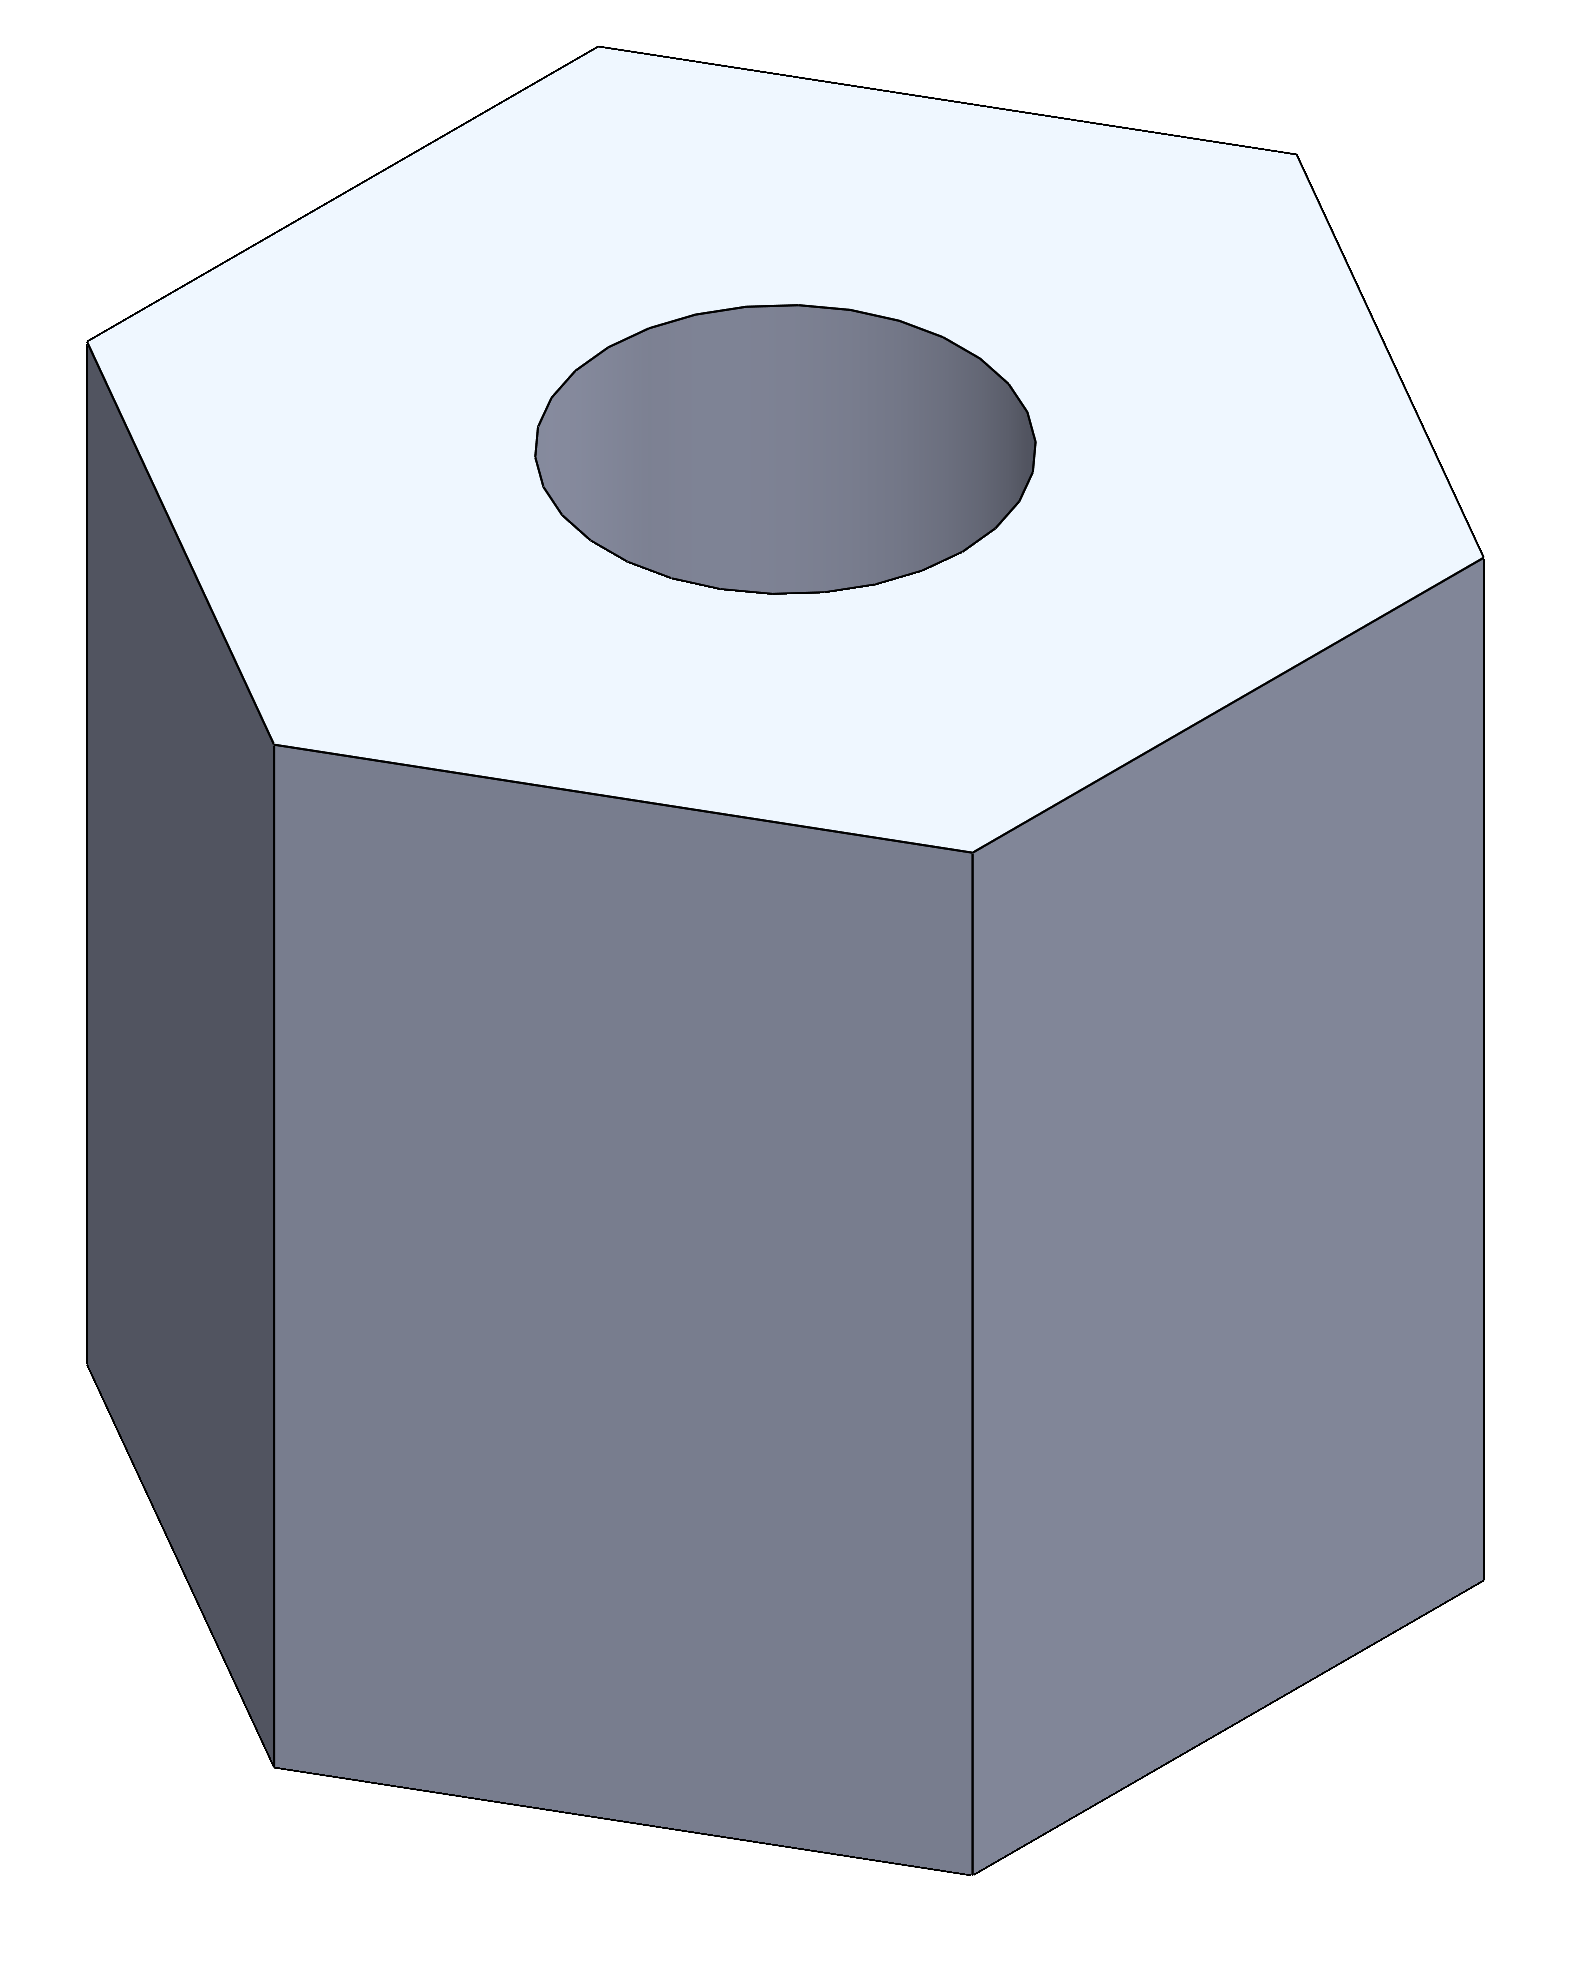
\includegraphics[width=\linewidth]{figures/parts/nut.PNG}
        \scriptsize Nut
      \end{minipage} &
      \begin{minipage}{0.3\linewidth}
        \centering
        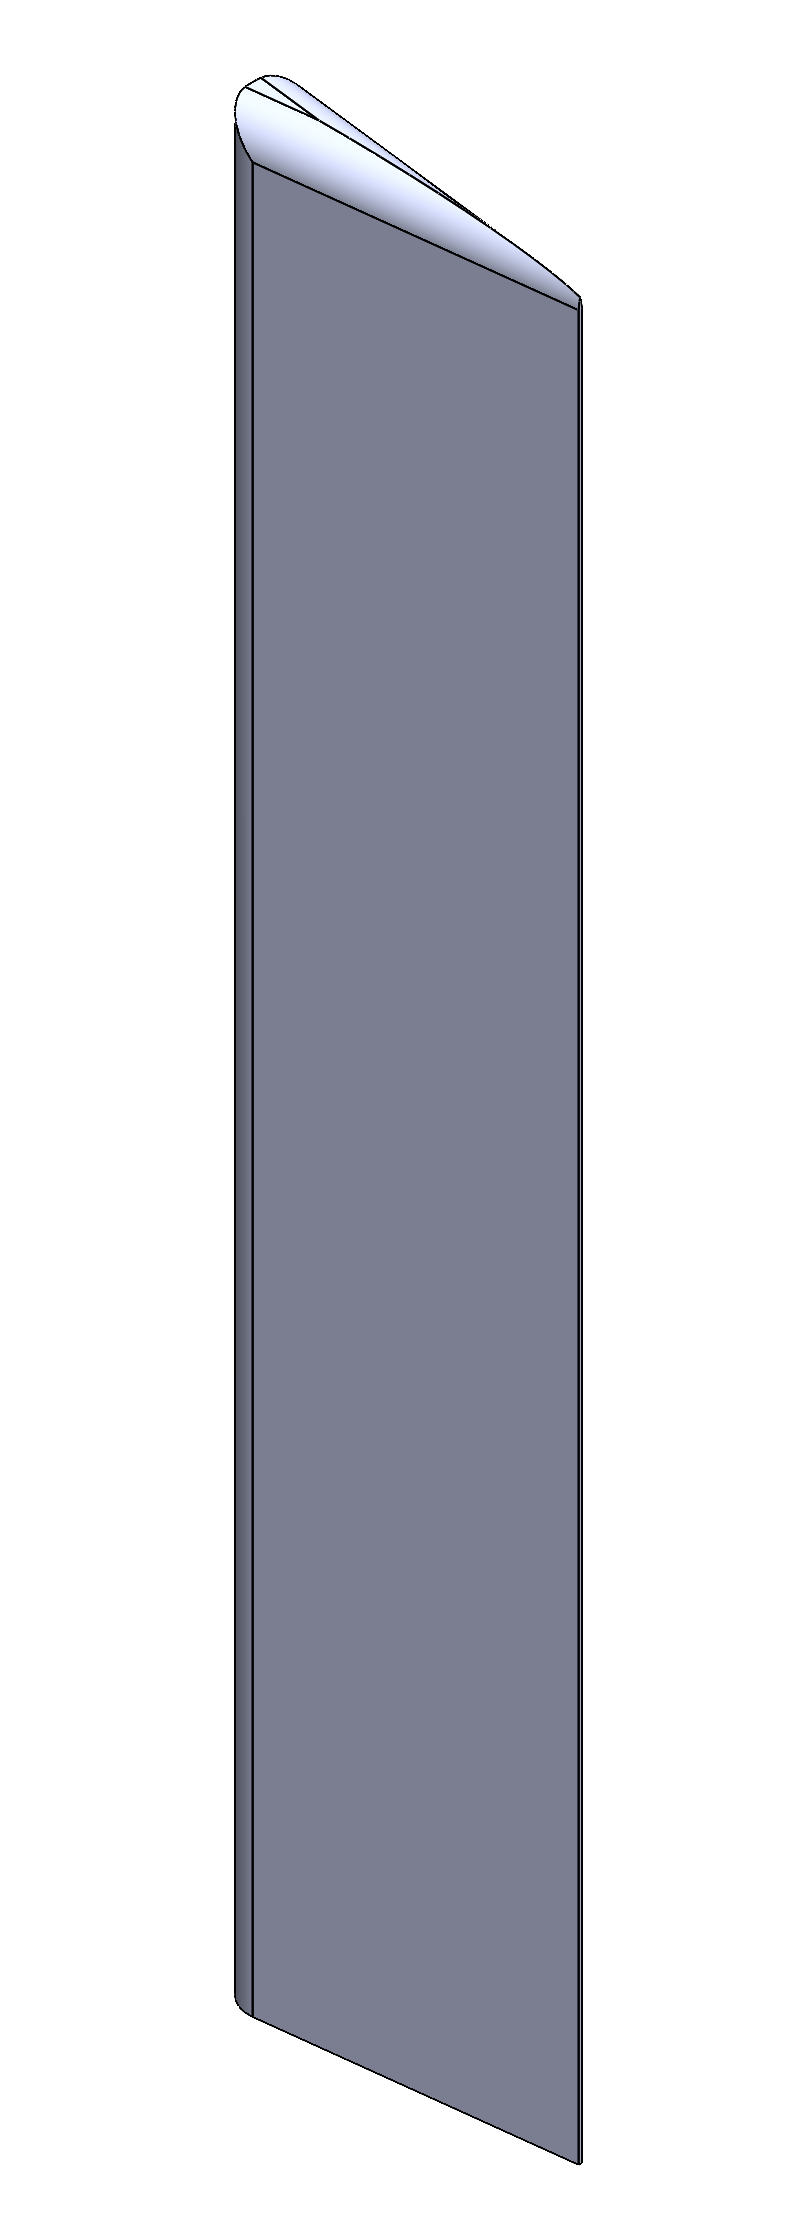
\includegraphics[width=\linewidth]{figures/parts/wedge.PNG}
        \scriptsize Wedge
      \end{minipage} &
      % Last column left blank
      \begin{minipage}{0.3\linewidth} \end{minipage} \\
    \end{tabular}
  \end{minipage}

  \caption{Shapes used in the dataset for MLP training.}\label{fig:part_shapes_grid}
\end{figure}













